\label{SemiWalkerDeltaConstellations}
As discussed in the report, Semi Walker Delta Constellations (SWDC) are a type of constellations in which the ascending nodes of each orbital plane are evenly spaced across 180 degrees.

\begin{figure}[H]
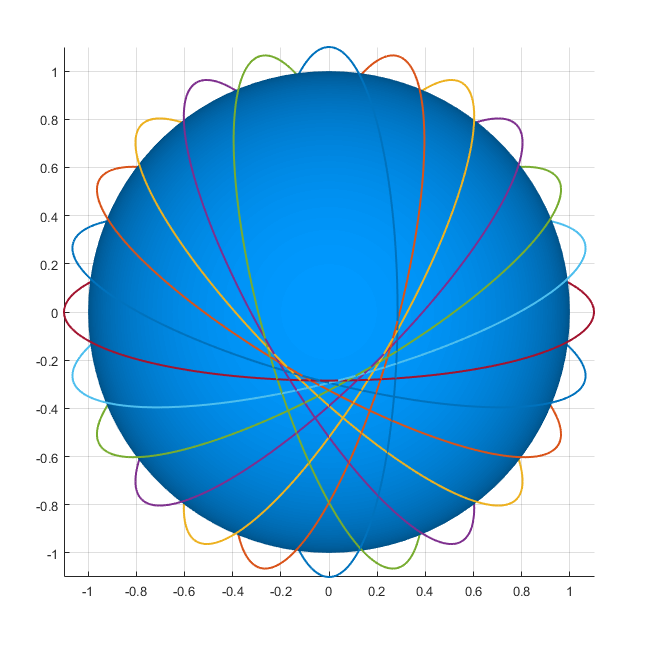
\includegraphics[width=12cm]{semiwalker12vertical}
\centering
\caption{12 plane SWDC. Note the gap and the equidistant planes}
\end{figure}

\subsubsection{Advantages}
\begin{itemize}[label={--}]
\item\textbf{Distance between planes reduced.} With the SWDC constellation the redundant orbits are directly corrected, thus the distance between planes is reduced to half, as results from the geometry itself.
\item\textbf{Less number of planes needed.} This means that in order to approach global coverage fewer planes will be requiered due to the decrease in distance between planes.
\item\textbf{Satellites following the same direction - sense.} With the SWDC constellation the orbits have no interaction with each other, thus the satellites for each orbit can be set following the same direction. This will significantly improve the communications among satellites from different planes; also, we will be avoiding the Doppler Effect.
\end{itemize}

\begin{figure}[H]
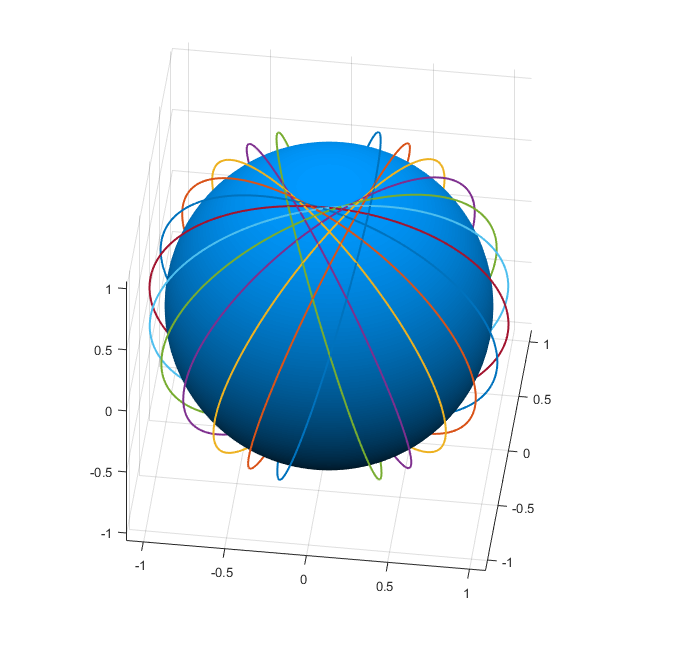
\includegraphics[width=12cm]{semiwalker12}
\centering
\caption{This geometry distribution induces a large anti-symmetric gap}
\end{figure}

\subsubsection{Disadvantages}
\begin{itemize}[label={--}]
\item\textbf{Gap configuration.} With the SWDC constellation, the main problem is the gap that results from configuring the constellation at a given inclination and describing equidistant orbits. In order to fulfill global coverage this gap will have to be covered by means of auxiliar orbits.
\end{itemize}

\subsubsection{SWDC including an additional polar orbit.}
As we have discussed for the SWDC, the main disadvantage respect to the Walker Delta Configuration is the fact that a gap is obtained, thus a global coverage network cannot be described. In order to cover the entire Earth we have analysed some ways of covering the gap with auxiliar orbits.

The most simple way would be to add a polar orbital plane. This polar orbit would be set directly on top of the gap described by the SWDC. The main issue with polar orbits, as discussed before in this report, is the complex reorientation and decay in inclination that takes place.

\begin{figure}[H]
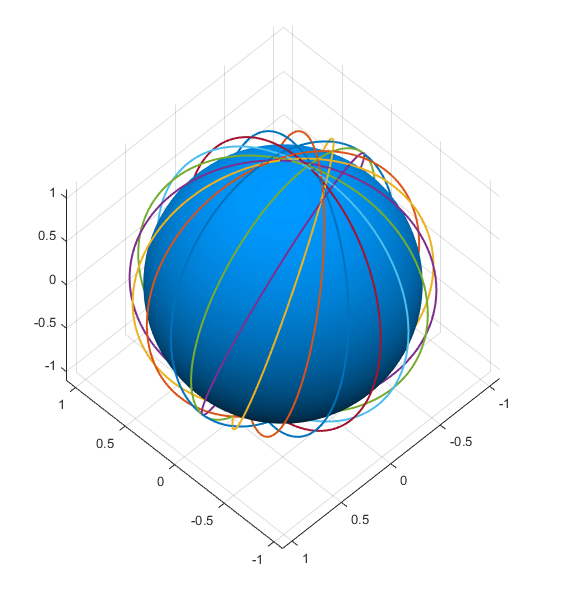
\includegraphics[width=10cm]{semiwalker11p1}
\centering
\caption{Added polar orbit to the 11 plane based SWDC}
\end{figure}

Moreover, in a Walker Delta Constellation, since all orbits have the same inclination, same height, and the planes are evenly spaced, the orbit perturbations are equal on each orbit and the constellation keeps its original shape. If a polar orbit is inserted in the constellation, the perturbations will be different than on the other orbital planes and the constellation will lose its initial configuration. Therefore, this solution is not suitable for our constellation and is discarded.